\section{Trilinear plots}\label{sec:twoway-trilinear}
The \glossterm{trilinear plot}
(also called a \emph{ternary diagram} or \emph{trinomial plot})
is a specialized display for a 3-column \ctab{} or for
three variables whose relative proportions are to be displayed.
Individuals may be assigned to one of three diagnostic categories,
for example, or a chemical process may yield three constituents
in varying proportions, or we may look at the division of votes
among three parties in a parliamentary election.
This display is useful, therefore, for both frequencies
and proportions.
Trilinear plots are featured prominently in \citet{Aitchison:86},
who describes statistical models for this type of
\glossterm{compositional data}.  \citet{Upton:76,Upton:94}
uses them in detailed analyses of spatial and temporal changes in
British general elections.
\citet{Wainer:96} reviews a variety of other uses of trilinear
plots and applies them to aid in understanding the distributions
of students achievement in the
National Assessment of Educational Progress,
making some aesthetic improvements to the traditional form of these
plots along the way.

A trilinear plot displays each observation as a point inside
an equilateral triangle whose coordinate corresponds to the
relative proportions in each column.
The three vertices represent the three extremes when 100\%
occurs in one of the three columns; a point in the exact
center corresponds to equal proportions of $\frac13$ in
all three columns.  For instance, \figref{fig:tripdemo2}
shows how three points whose compositions of three variables,
A, B, and C are shown as annotations.
Note that each apex corresponds to 100\% of the labeled
variable, and the percentage of this variable decrease
linearly along a line to the midpoint of the opposite
baseline.
The grid lines in the figure show the percentage value along
each axis.

\begin{figure}[htb]
  \centering
  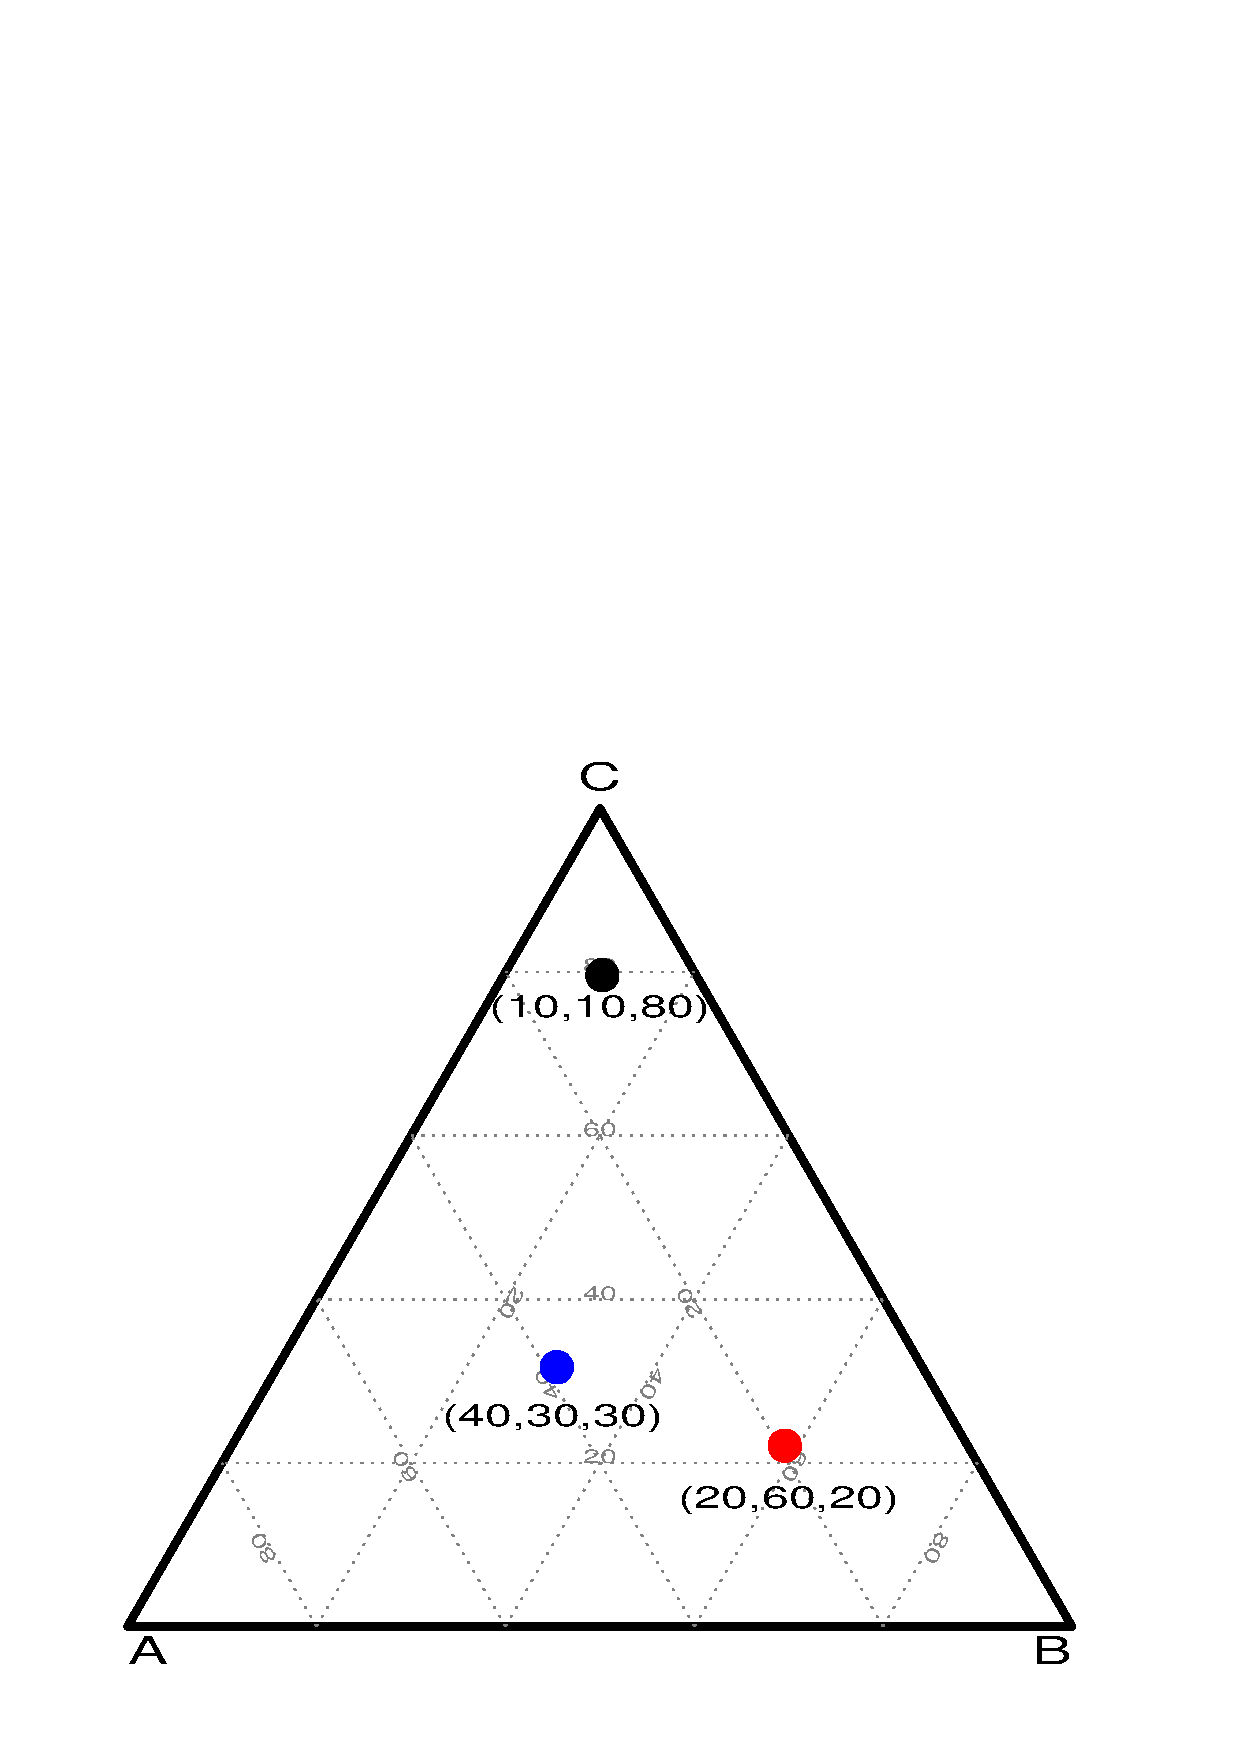
\includegraphics[scale=.6]{ch3/fig/tripdemo2}
  \caption[A trilinear plot]{An illustrative trilinear plot}\label{fig:tripdemo2}
\end{figure}

The construction of trilinear plots is described in detail
by \citet{FedenczukBercov:91}.
Briefly, let $P(a, b, c)$ represent the three components  normalized so
that $a + b + c = 1.0$.
If the apex corresponding to Point A in \figref{fig:tripdemo2}
is given $(x, y)$ coordinates of $(x_A, y_A) = (0, 0)$,
and those at apex B are $(x_B, y_B) = (100, 0)$,
then the coordinates of apex C are $(x_C, y_C) = (50, 50\sqrt{3})$.
The coordinates $(x_P, y_P)$  of $P$ are then calculated as
\begin{eqnarray*}
y_P & = & c \: y_C \\
x_P & = & y_P \left( \frac{y_C - y_B}{x_C - x_B} \right)
+ \frac{\sqrt{3}}{2} y_C (1 - a) \\
\end{eqnarray*}

The figures shown here are produced using the \macro{TRIPLOT},
which is listed in \macref{mac:triplot}.

\begin{Example}[arthrit5]{Arthritis treatment}
%\example{Arthritis treatment}
In the Arthritis treatment data, our interest is focused on the
relative numbers of individuals in the three outcome categories
for the four groups defined by the combinations of Treatment
and Sex.

\figref{fig:arthtri} shows clearly that both groups given the
active treatment result in greater proportions of successful
outcomes (some or marked improvement) than do the placebo
groups.
In addition, regardless of treatment, females show greater
proportions of successful outcomes than do males.

\begin{figure}[htb]
  \centering
  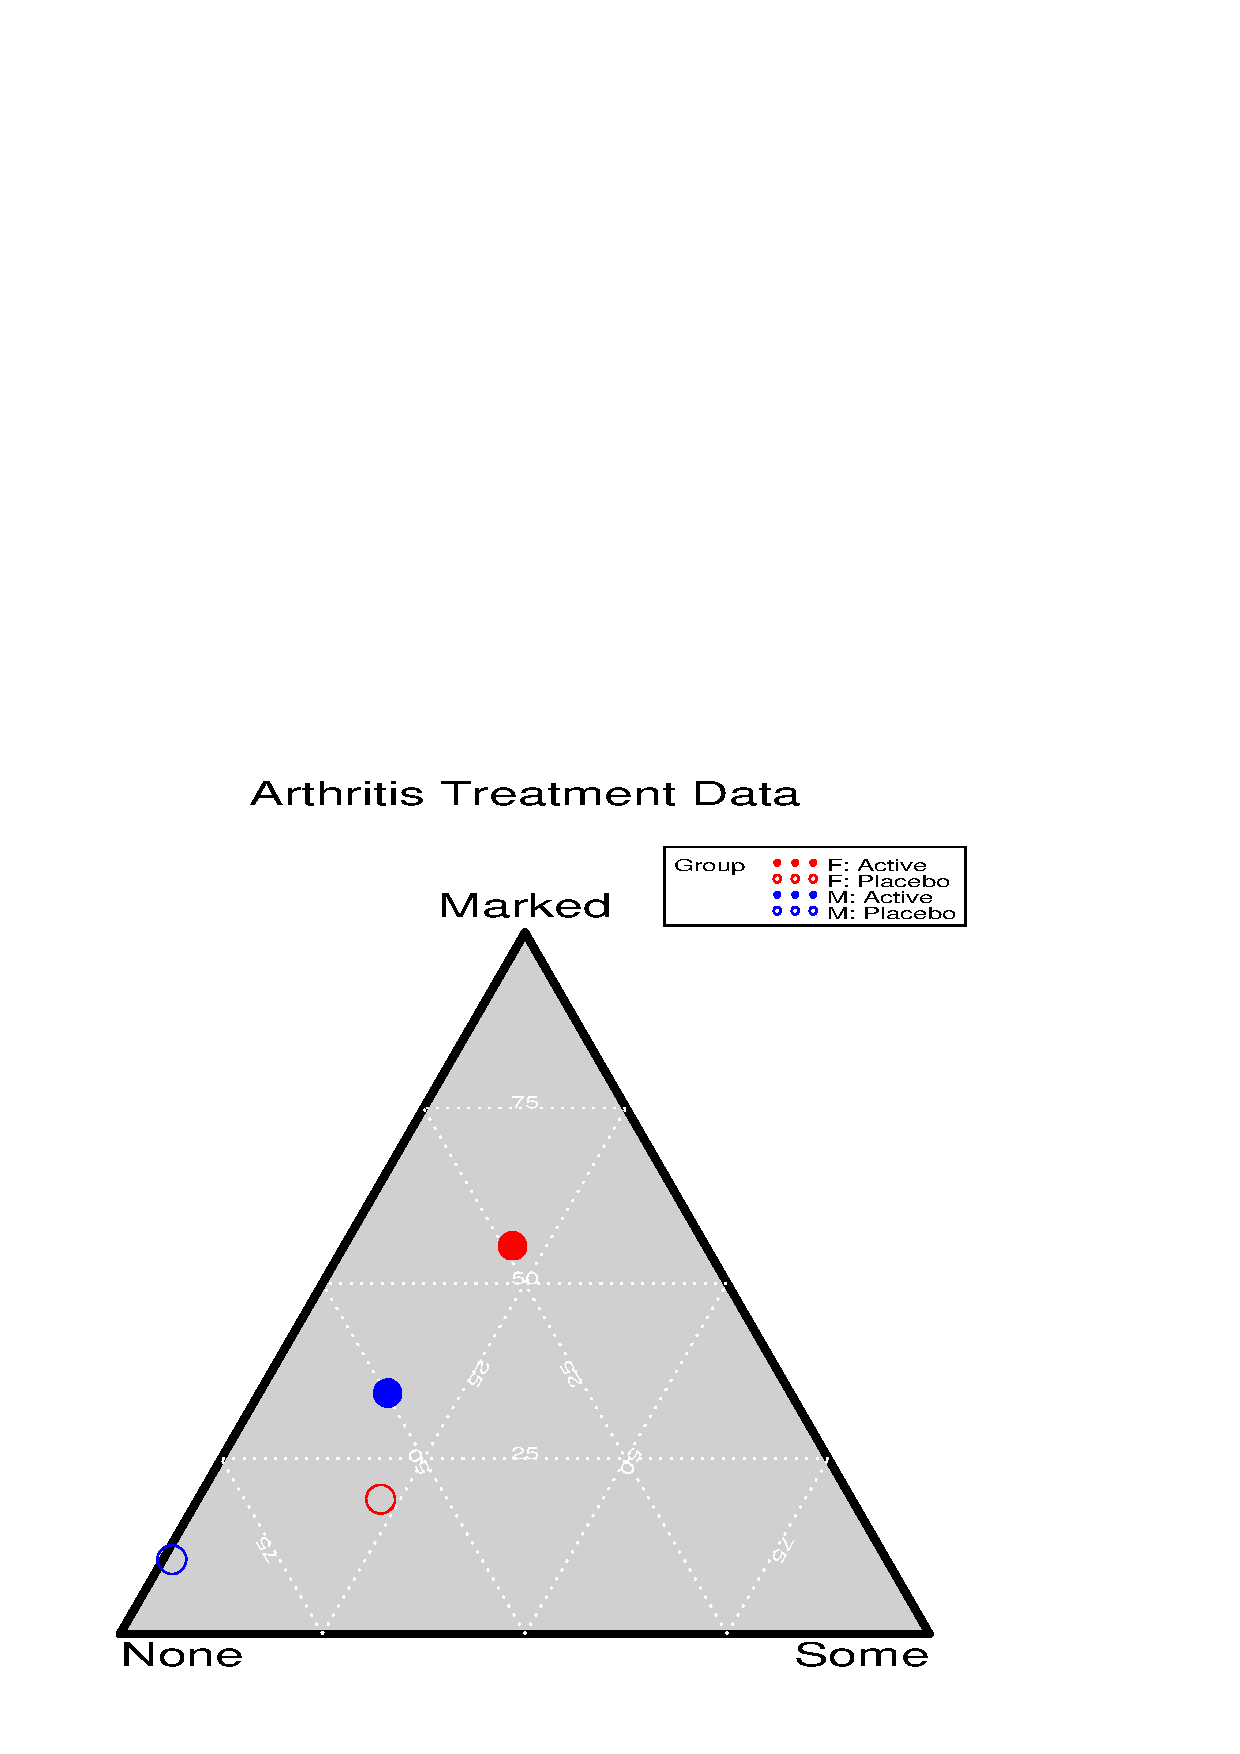
\includegraphics[scale=.6]{ch3/fig/arthtri}
  \caption[Trilinear plot for Arthritis treatment data]{Trilinear plot for Arthritis treatment data}\label{fig:arthtri}
\end{figure}

\figref{fig:arthtri} is produced using the \macro{TRIPLOT}
as follows.  For convenience in identifying the treatment-sex combinations,
these two variables are combined into a single \texttt{GROUP} variable,
used as the value of the \texttt{CLASS=} parameter in the macro call.
%% input: /users/faculty/friendly/sasuser/catdata/arthtri.sas
%% last modified: 14-Jan-98 14:02
\begin{listing}
title 'Arthritis Treatment Data';
data arth;
   input sex $ treat $ @;
   input none some marked;
   length group $10;
   sex = substr(sex,1,1);
   group = trim(sex) || ': ' || treat;
   label group='Group';
datalines;
Female  Active    6  5  16
Female  Placebo  19  7   6
Male    Active    7  2   5
Male    Placebo  10  0   1
;
%triplot(data=arth,
   var=None Some Marked, class=group,
   symht=4, 
   symbols=dot circle dot circle,
   colors=red red blue blue, 
   backclr=grayd0, backpat=solid,
   gridclr=white, gridby=25);
\end{listing}

\end{Example}

\begin{Example}[baseball]{Baseball fielding}
The \emph{Baseball \Dset} from \SSSGref{A2.3}
includes data on the salaries and batting and fielding performance of 322 major league in the 1986 baseball season.
Fielding performance includes the numbers of Errors,
Putouts and Assists made by each player.
(Putouts occur when a fielder causes an opposing player to be tagged or forced out;
assists are credited to other fielders involved in making that
putout.)

\figref{fig:basetri} shows a triplot for this data.
Because of the large number of observations in the \Dset,
the mean number of putouts, assists and errors was calculated for each team
and for each position, giving a reduced \Dset\ of 169 observations.%
\footnote{Putouts and assists also occur far more often than errors,
so the values of each variable were also first scaled to a common range.}
These observations are graphed in \figref{fig:basetri} coding the
player's position by the plotting symbol.

\begin{figure}[htb]
  \centering
  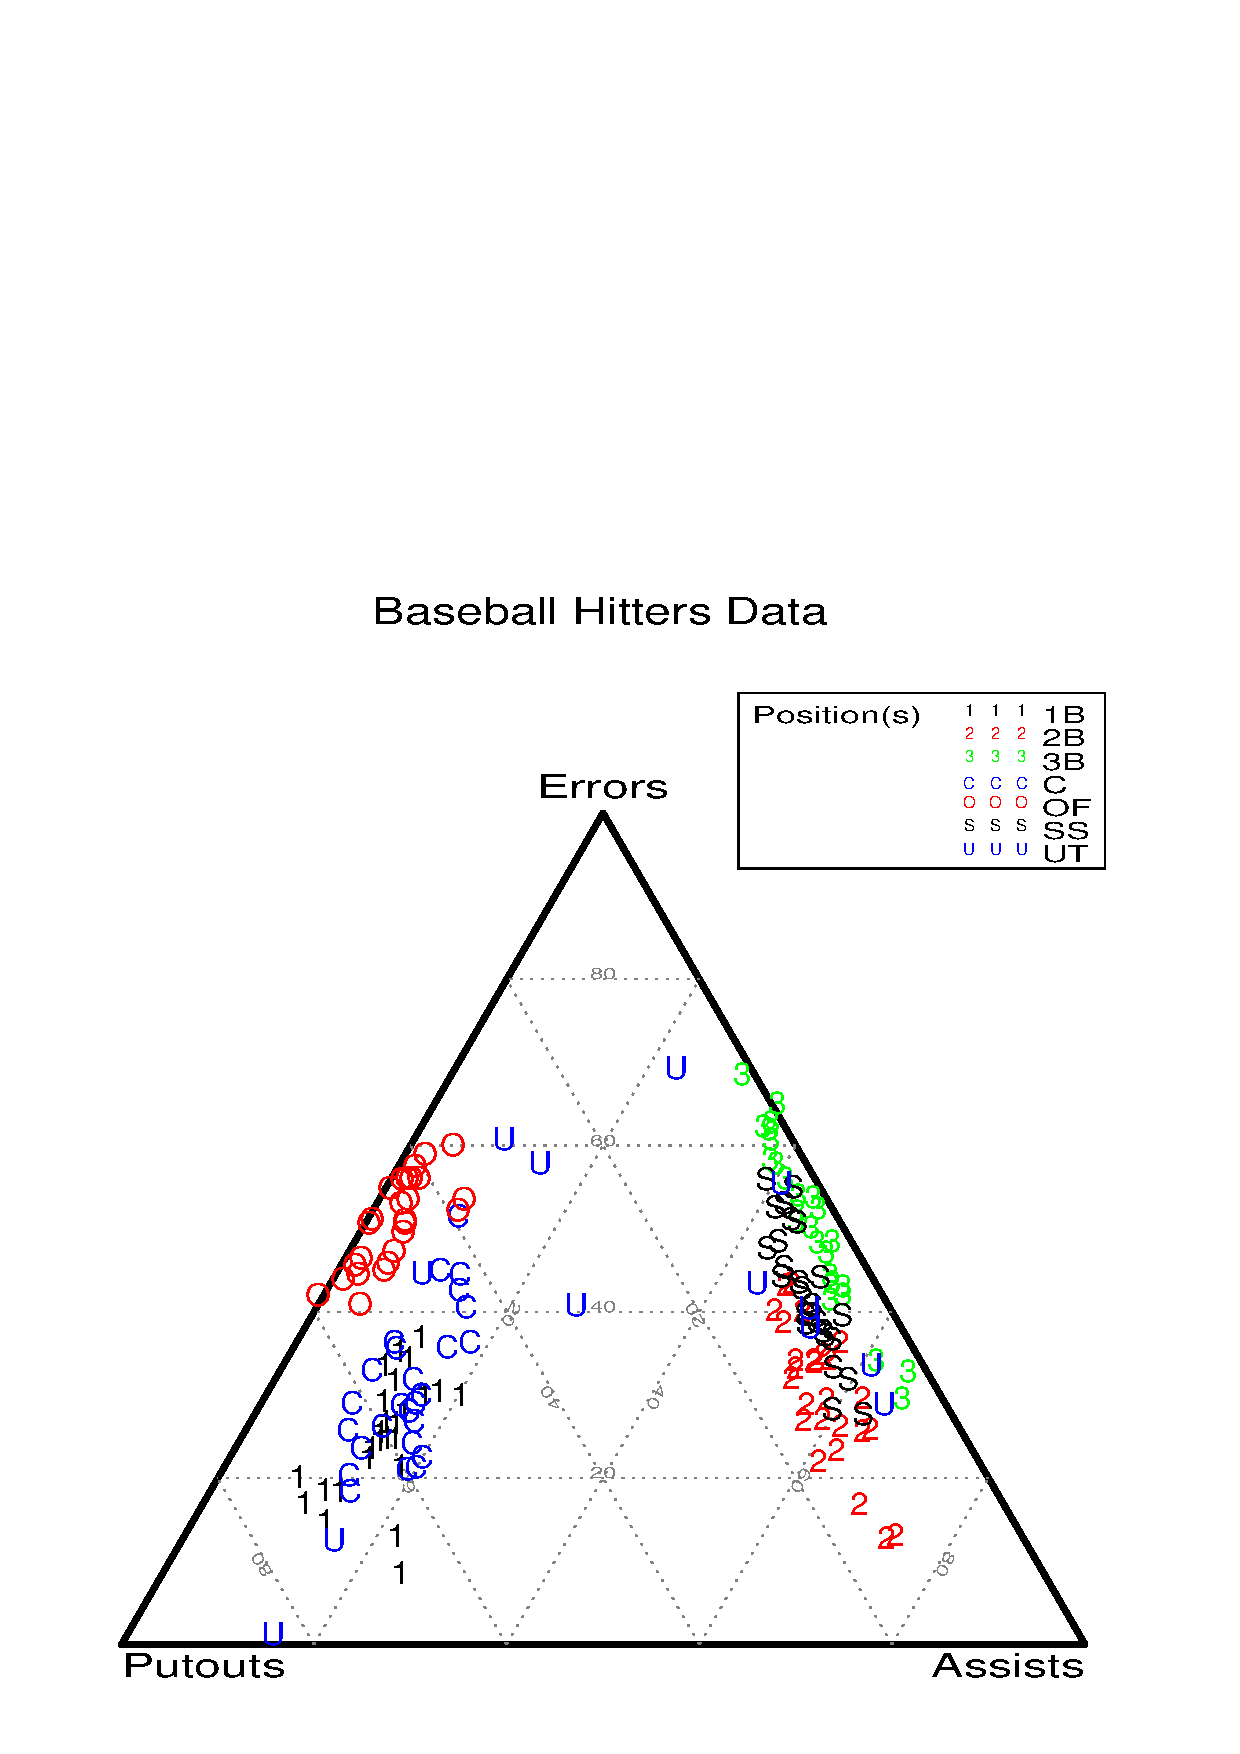
\includegraphics[scale=.6]{ch3/fig/basetri}
  \caption[Trilinear plot for baseball data]{Trilinear plot for baseball fielding data}\label{fig:basetri}
\end{figure}

It may be seen that two main types of
players may be distinguished by their relative proportions of
putouts and assists: Outfielders, catchers and first basemen
contribute to defense primarily in making putouts; other infielders
primarily make assists.  The utility players (UT) play in a variety
of positions and are scattered throughout the plot.
Beyond this main observation, you can also see that outfielders and
third basemen tend to make more errors than players in other positions.
\end{Example}

\begin{Example}[lifeboat1]{Lifeboats on the \emph{Titanic}}
We examine the question of who survived and why in the sinking of the \emph{RMS Titanic} in \secref{sec:mosaic-threeway} (\exref{ex:titanic}),
where we analyze a four-way table of the 2201 people on board (1316 passengers and 885 crew),
classified by Class, Sex, Age, and Survival.
A different \Dset\ which sheds some light on the same issues is
appropriate here.

After the disaster, the British Board of Trade launched several
inquiries, the most comprehensive of which resulted in the
\emph{Report on the Loss of the ``Titanic'' (S.S.)}
by Lord Mersey
\citep{Mersey:1912}.
Section 4 of this document contains a detailed account of the saving
and rescue of the passengers and crew who survived.
The \emph{Titanic} was outfitted with 20 boats, half on each of the
port and starboard sides,
 of which 14 were large
lifeboats with a capacity of 65, two were emergency boats designed for
40 persons, and the remaining four were collapsible boats capable of holding
47, a total capacity of 1178 (considered adequate at that time).
Two of the collapsible boats, lashed to the roof of the officers
quarters, were ineffectively launched and utilized as rafts after the ship sunk.
The report lists the time of launch and composition of the remaining 18 boats according to male passengers, women and children, and ``men of crew'',
as reported by witnesses.
The \Dset\ \texttt{lifeboat} (see \datref{dat:lifeboat})
contains the data listed on p. 38 of that report.%
\footnote{The ``data'' lists a total of 854 in 18 boats, although only
712 were in fact saved.  Mersey notes ``it is obvious that these figures
are quite unreliable''.  Allowing for 60 people rescued from the water,
only 652 could have left in the boats \citep[p. 39]{Mersey:1912}.
We present an alternative \Dset, \pname{LIFEBOA2}, in \datref{dat:lifeboat},
based on more conservative and historically accurate informatio.}

Of interest here is the composition of the boats by these three categories
and according to the launching of the boats from the port or starboard
side, which can be shown in a trilinear display
using the following statements.
The parameter \pname{idsubset = men>.1} is used to label only boats
in which the proportion of male passengers exceeded 10\%.
(The values of variables have been scaled to sum to 1.0 for each observation
at the time the \mparm{idsubset}{TRIPLOT} is used.)
The \pname{labloc=0} parameter is used to label the axes at the value
corresponding to 0\%
rather than at the vertex (\pname{labloc=100}) as in the earlier plots.

\begin{listing}
legend1  position=(top right inside) across=1
   offset=(0,-25pct) mode=share frame;
%triplot(data=lifeboat,
   var=Crew Men Women,
   id=boat, class=side,
   legend=legend1, labloc=0,
   idht=1.7, symht=1.7,
   idsubset=men>.1,
   symbols= circle dot, colors=red blue);
\end{listing}
\begin{figure}[htb]
  \centering
  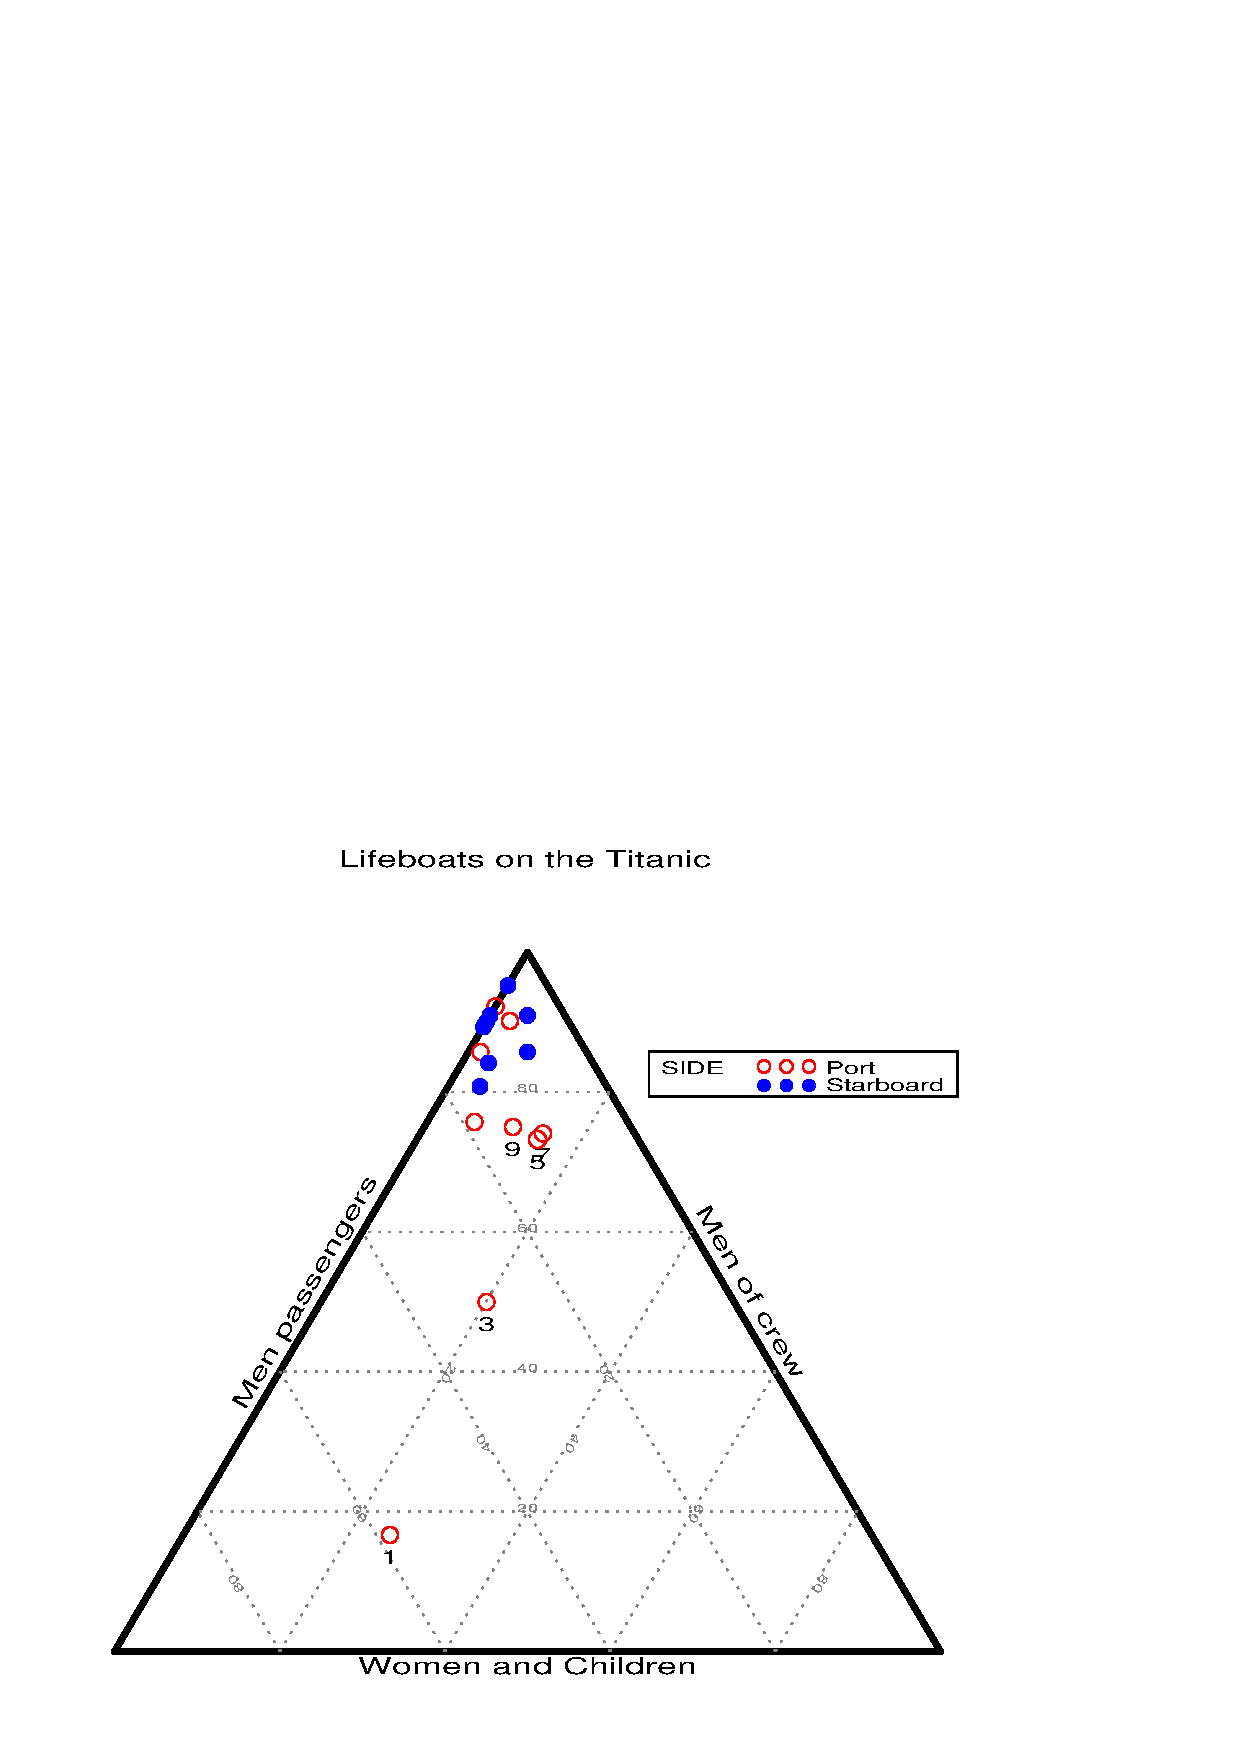
\includegraphics[scale=.6]{ch3/fig/lifeboat1}
  \caption[Lifeboats on the \emph{Titanic}]{Lifeboats on the \emph{Titanic},
  showing the composition of each boat.  Boats with more than 10\% male
  passengers are labeled.}%
  \label{fig:lifeboat1}
\end{figure}

The result, shown in \figref{fig:lifeboat1}, makes it immediately apparent
that many of the boats launched from the port side differ substantially
from the remaining boats, whose passengers were almost entirely women
and children.  Boat 1 had only 20\% (2 out of 10) women and children, while the percentage for boat 3 was only 50\% (25 out of 50).


The triplot scales the numbers for each observation to sum to 1.0,
so differences in the total number of people on each boat
cannot be seen in \figref{fig:lifeboat1}.
The total number reported loaded is plotted against launch time in \figref{fig:lifeboat2},
with a separate regression line fit to the data for the port and starboard
sides.
It seems clear that the rescue effort began in panic on the port side,
with relatively small numbers loaded, and (from \figref{fig:lifeboat1}),
small proportions of women and children.
But the loading regime improved steadily over time.
The procedures began more efficiently on the starboard side
and the numbers loaded increased only slightly, though still
with large variability from boat to boat.
\begin{figure}[htb]
  \centering
  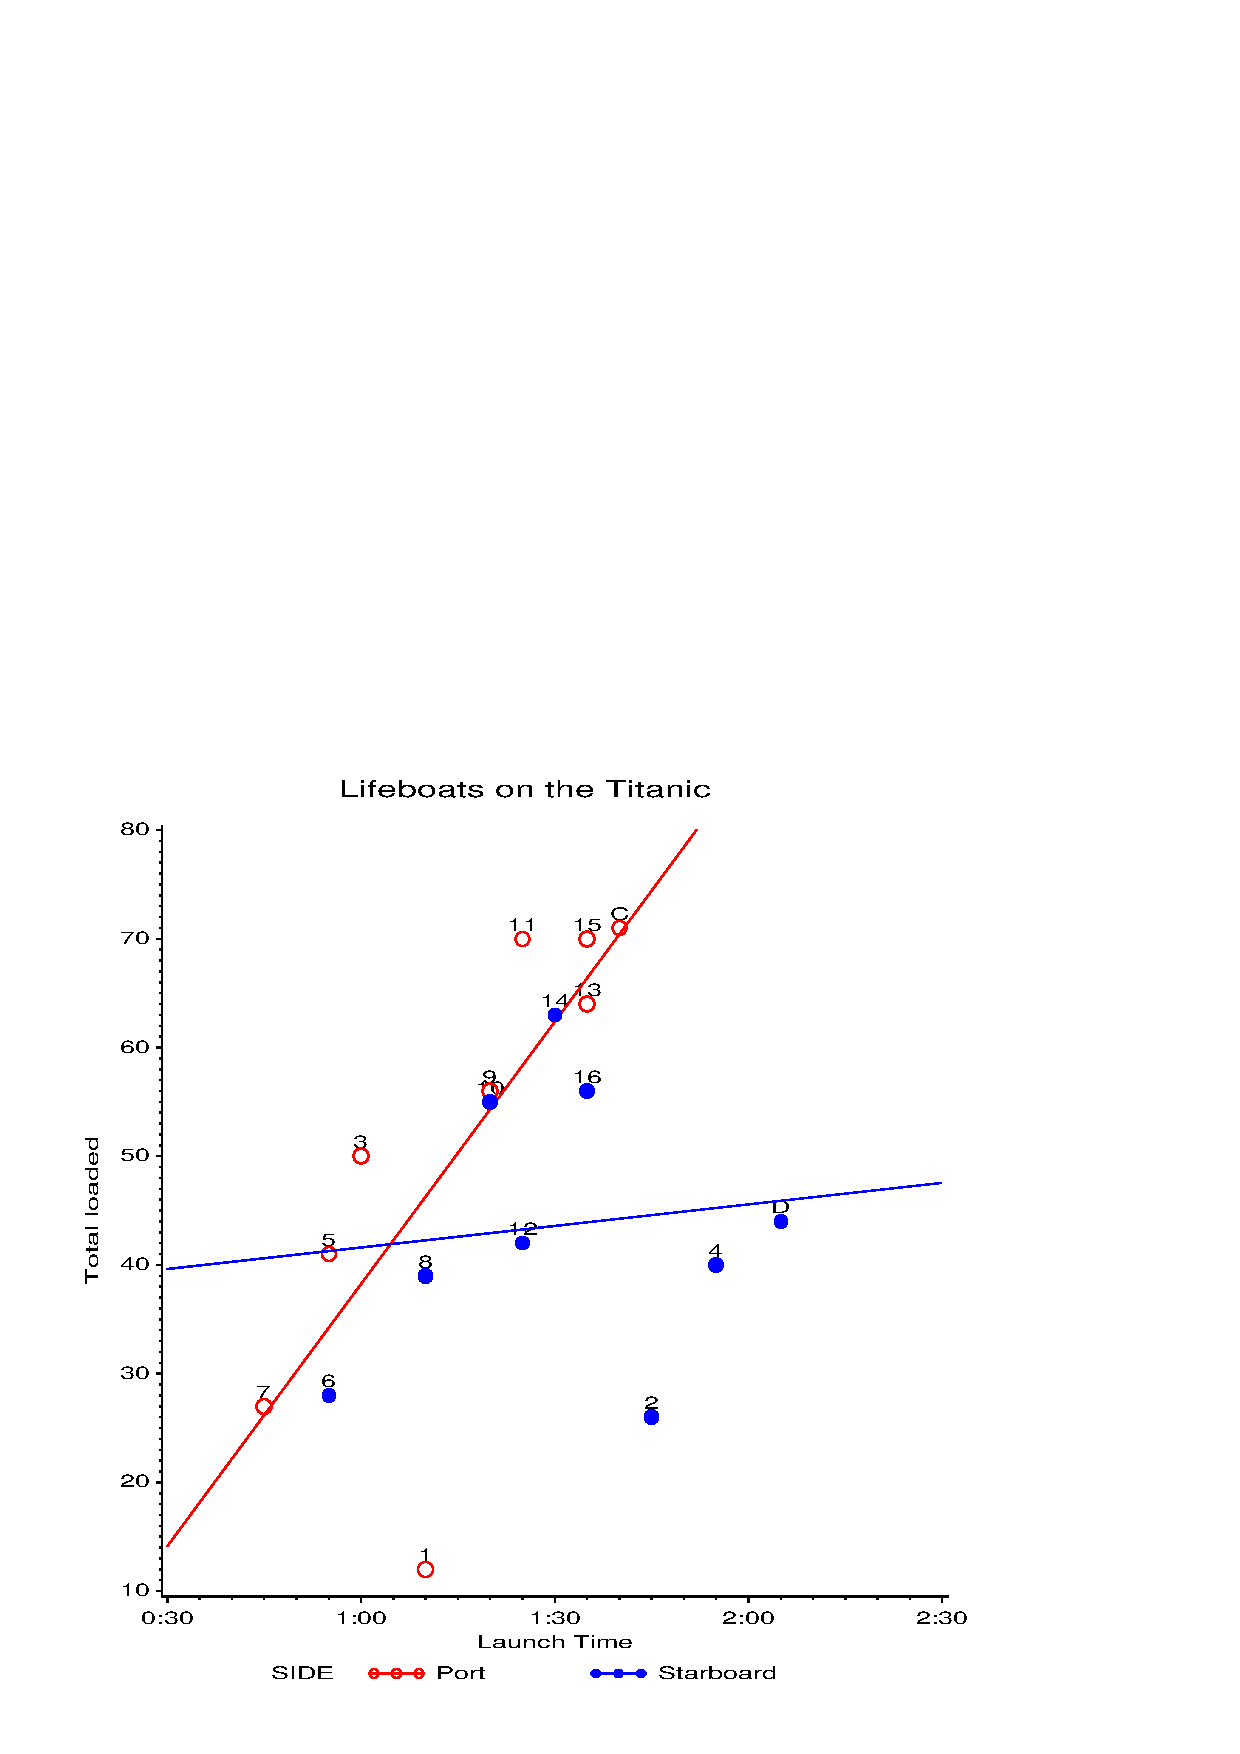
\includegraphics[scale=.6]{ch3/fig/lifeboat2}
  \caption[Lifeboats on the \emph{Titanic}]{Lifeboats on the \emph{Titanic},
  showing the numbers loaded on each boat.
  Regression lines for each side indicate a difference in regimes for
  the port and starboard sides.}%
  \label{fig:lifeboat2}
\end{figure}
\end{Example}

